In the previous chapter, we have introduced some background on statistics and
optimization.
In this chapter, we present the necessary background on the data used in this
thesis.
In our experiments we use functional magnetic resonance imaging (fMRI) or
magnetoencephalograpy (MEG) data. As will be seen in this chapter, these two modalities have very different
characteristics.

\section{Functional magnetic resonance imaging (fMRI)}
This section summarizes information borrowed from the handbook of fMRI data analysis~\cite{poldrack2011handbook}.

\subsection{The BOLD signal and hemodynamic response}
The story of fMRI begins with the discovery of the blood-oxygen-level-dependent
(BOLD) imaging contrast in 1990 by Ogawa~\cite{ogawa1990brain}. When neurons
fire, they consume oxygen and therefore, the level of oxygen in blood changes (it is actually over-compensated by blood supply).
Since oxygenated and deoxygenated blood (oxyhemoglobin
and deoxyhemoglobin) do not have the same magnetic susceptibility, changes in
the oxygen level in blood can be tracked by a magnetic resonance imaging (MRI) scanner.

When a short stimuli occurs, the change in the relative change in the MRI signal (BOLD
signal) is not instantaneous. The typical response to a stimuli follows the
curve displayed in figure~\ref{fig:hrf}. This response is rather slow (it may last \emph{20s}) compared to the temporal scale of neurons which is on the order of \emph{ms}.

\begin{figure}
  \center
  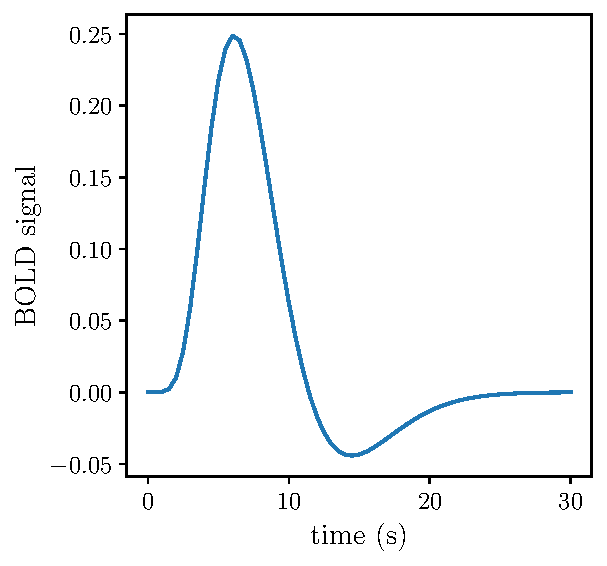
\includegraphics[scale=0.8]{figures/neuroscience/hrf.pdf}
  \caption{A model of the hemodynamic response function}
  \label{fig:hrf}
\end{figure}

Luckily, the shape of the hemodynamic response does not vary much across time
and therefore the BOLD signal is often seen as the result of the convolution of neural activation with the hemodynamic response.

\subsection{Spatial and temporal resolution of fMRI data}
The success of fMRI is due to its advantages compared to positron
emission topography (PET) that uses radioactive tracers to follow glucose or water levels.
While PET has a spatial resolution of a few
centimeters, fMRI has a spatial resolution of a few millimeters. As a result, a voxel in an fMRI image typically encompasses several hundreds thousands of neurons.
In addition, while taking an image with PET takes about a minute, it takes on the order of 2s to produce a full-brain fMRI image.
Lastly, fMRI is non-invasive and does involve being exposed to radioactive tracers as in PET.

\subsection{Experimental designs}
In \emph{resting state} fMRI, subjects are instructed to lie still in the scanner without further instruction.
This kind of data can be used to extract networks that highlight sets of regions that tend to co-activate.
This contrasts with \emph{task} fMRI, where subjects follow specific instructions.
In task fMRI, two types of experimental design are widespread.
Block designs are widespread designs particularly suited to modalities with low temporal resolutions (such as PET). In block designs, subjects are exposed to continuous stimuli that last of a rather long period of time before it switches to another.
This contrasts with event related designs that are only suited to modalities with a finer time resolution. In event related design, a sequence of short event are presented and separated by a time window (inter-stimulus interval).
When the inter-stimulus interval is shorter than the length of the hemodynamic response, we talk about ``fast'' even related designs.
Lastly, in \emph{naturalistic fMRI}, subjects are instructed to watch a movie
or listen to an audio track. These kinds of stimuli are called \emph{naturalistic stimuli} and constitue a middle ground between resting state and task fMRI as activations are time locked while the environment is not as controlled as in a typical task fMRI setting.
%
In this thesis, we use mostly \emph{naturalistic fMRI}, as one of our motivations is to propose a suitable framework to analyse such data.

\subsection{Preprocessing}
The fMRI signal is particularly noisy. Several techniques are used to reduce the noise and enhance the quality of the data.

\subsubsection{Distortion correction}
In the MRI scanner, a constant magnetic field is applied. However, in areas
where an air/tissue interface, the magnetic field is distorted leading to errors in
the localization of voxels near the sinus or ears. However, most scanners come
with a map quantifying the distance that each voxel has been shifted. By
inverting the map, one can try and recover the correct location of voxels.


\subsubsection{Slice timing correction}
Images are acquired in slices, a few slices at a time, so that different voxels are acquired at different times.
In order to correct for this effect, a reference slice is chosen and other slices are interpolated so that all the voxels can be considered to have been acquired at the same time. 

\subsubsection{Motion correction}
Head motion causes massive distortion of the signal. Such effects are corrected by
chosing a reference image and apply rigid body transformations so that other
images match the orientation and localization of the reference image. One also records estimated head movements parameters so that they can be regressed out. However, if the task is correlated with head motion, this regression can destroy signal.

\subsubsection{Spatial smoothing}
Spatial smoothing blurs the image by application of a Gaussian kernel with a given width (in mm). When the signal of interest has a large spatial extend, smoothing increases the signal to noise ratio. 
Smoothing is also used as a way to decrease between subject variability.
In our experiment, we usually don't apply smoothing in order to measure how our
methods are able to handle fined grained details. While there is currently no
consensus on smoothing, we observe that a smoothing of 3~mm generally improves
most analysis on fMRI data.

\subsubsection{Frequency filtering}
Heating of the scanner causes a low temporal frequency noise to appear. In order
to remove such noise, a high pass filtering is applied with a cut-off frequency
of $0.01 Hz$. Sometimes a low pass filter with a cut-off frequency of $0.1$ Hz is also used since artifacts induced by motion are usually of higher frequency than the signal of interest.

\subsubsection{Spatial normalization}
Each subject has a brain of different size and of different shape.
The goal of spatial normalization is to align the subjects in order to reduce anatomical variability.
The most widespread technique is to align all images on a template image. The
template image used is based on an atlas developed at the Montreal Neurological
Institute (MNI atlas) where 305 anatomical images were aligned, averaged and then re-aligned to the mean image based on an non-linear registration model.
An affine linear registration is applied, followed by non-linear deformation to better match brain shape. Typically, fMRI images of each subject are aligned on a high dimensional anatomical image of the same subject (this step is called \emph{coregistration}) and then the anatomical image is aligned to the MNI atlas. The two transformations are then composed to project fMRI data to the MNI space.

\subsubsection{Masking}
It is often the case that only a subpart of the brain is of interest. When this is the case, we use a mask to only keep the set of voxels corresponding to particular locations defined by the mask.

\subsubsection{Runs}
For the comfort of participants and to ensure their active participation, it is in general not possible to use the scanner without interruptions for more than 10 minutes.  When long acquisitions must be
performed they are split into short runs of approximately 10 minutes.


\subsection{Example of fMRI Datasets}
\label{srm:datasets:fmri}
In this subsection we provide examples of fMRI datasets. These datasets will be used to evaluate the methods developed in this thesis.
Datasets are preprocessed with FSL \url{http://fsl.fmrib.ox.ac.uk/fsl}  and SPM \url{https://www.fil.ion.ucl.ac.uk/spm/software} using slice timing correction, distortion correction spatial realignment, coregistration to the T1 image and affine transformation of the functional volumes to a template brain (MNI).
Using Nilearn \cite{abraham2014machine}, preprocessed data are masked (using a full brain mask available at
\url{http://cogspaces.github.io/assets/data/hcp_mask.nii.gz}), detrended and
standardized (so that any voxel's timecourse has zero mean and unit variance).
We also apply a high pass filter and a low pass filter with cut-off frequencies of 0.01 Hz and 0.1 Hz respectively).

In the \emph{SHERLOCK} dataset, 17 participants are watching "Sherlock" BBC TV show (episode 1). 
% 
These data are downloaded from \url{http://arks.princeton.edu/ark:/88435/dsp01nz8062179}. 
% 
Data were acquired using a 3T scanner with an isotropic spatial resolution of 3~mm. 
% 
More information including the preprocessing pipeline is available in \cite{sherlock}.
% 
Subject 5 is removed because of missing data, leaving us with 16 participants.
% 
Although SHERLOCK data contains originally only 1 run, we split it into 4 blocks of 395 timeframes and one block of 396 timeframes for the needs of our experiments. 

In the \emph{FORREST} dataset, 20 participants are listening to an audio version of the movie Forrest Gump.
% 
FORREST data are downloaded from OpenfMRI~\cite{poldrack2013toward}. 
% 
Data were acquired using a 7T scanner with an isotropic spatial resolution of 1 mm (see more details in \cite{hanke2014high}.
% 
More information about the forrest project can be found at \url{http://studyforrest.org}.
% 
Subject 10 and run 8 are discarded because of missing data.
% 
We therefore use full brain data of 19 subjects split in 7 runs of respectively 451, 441, 438, 488, 462, 439 and 542 timeframes.


In the fMRI \emph{CamCAN} dataset, 647 participants aged from 18 to 88 years are watching Alfred Hitchcock's "Bang! You're Dead" (edited so that it lasts only 8 minutes).
% 
CamCAN consists of data obtained from the CamCAN repository (available at \url{http://www.mrc-cbu.cam.ac.uk/datasets/camcan/}) (see \cite{taylor2017cambridge} and \cite{shafto2014cambridge}).
% 
We use all available subjects and runs yielding 647 participants and 1 run of 193 timeframes.


The \emph{RAIDERS} dataset reproduces the protocol described
in~\cite{haxby2011common}. 10 participants are watching the movie "Raiders
of the lost ark". This dataset pertains to the Individual Brain Charting
dataset~\cite{ibc, ibc2}.
% 
Data 
% 
We use full brain data of 10 subjects split in 9 runs of respectively 374, 297, 314, 379, 347, 346, 350, 353 and 211 timeframes.
%
Note that the Raiders dataset is different from the one used in~\cite{chen2015reduced}, as it involves different subjects, and because data were acquired at NeuroSpin using a 3T scanner with an isotropic spatial resolution of 1.5 mm.
The \emph{raiders-full} dataset~\cite{ibc, ibc2} is an extension of the \emph{raiders} dataset where the first two scenes of the movie are shown twice (130 mins).

The CLIPS dataset reproduces the protocol of original studies described in
\cite{nishimoto2011reconstructing} and \cite{huth2012continuous}. 10
participants are exposed to short clips. The data were acquired in 17 runs of 325 timeframes. 
%
The CLIPS dataset also pertains to the Individual Brain Charting dataset
(\cite{ibc, ibc2}).
%
At the time of writing, the CLIPS and RAIDERS dataset from the individual brain charting dataset \url{https://project.inria.fr/IBC/} are not yet public, but they will be in the future. Protocols on the visual stimuli presented are available in a dedicated repository on Github: \url{https://github.com/hbp-brain-charting/public_protocols}.

Unless stated otherwise we use spatially unsmoothed data, except for the
\emph{sherlock} dataset, for which the available data are already preprocessed
with a 6\,mm spatial smoothing. The temporal resolution or repetition time (TR) is 2s for all datasets except for the Sherlock dataset where the TR is 1.5s.
%

A summary about the size of each dataset is available in Table~\ref{tab:dataset_desc2}. Note in particular that all datasets have been resampled to 2mm isotropic resolution, leading to 212,445 voxels in the brain mask.
\begin{table}
	\begin{tabular}{|c|c|c|c|c|}
		\hline
		\textbf{Dataset} & \textbf{Subjects} & \textbf{Runs} & \textbf{Average run} & \textbf{Voxels} \\
                     && & \textbf{length} & \textbf{(per subject)} \\
                     && & \textbf{(in timeframes)} &  \\
                     &$m$& $ $ & $n$ &$v$  \\
		\hline
		CLIPS & 10 & 17 & 325 & 212445\\ 
		\hline
		SHERLOCK & 16 & 5 & 395 & 212445 \\ 
		\hline
		RAIDERS & 10 & 9 & 330 & 212445 \\
		\hline 
		FORREST & 19 & 7 & 465 & 212445\\
		\hline
		CamCAN & 647 & 1 & 193 & 212445 \\
		\hline
	\end{tabular}
  \caption{\textbf{Datasets description}}
  \label{tab:dataset_desc2}
\end{table}

\subsection{An example of univariate analysis: analyzing task fMRI data via the general linear model}
\label{sec:glm}
In this section, we describe a framework successfully applied to identify brain regions involved in specific tasks: the general linear model
(GLM)~\cite{friston1995analysis}. We refer the reader to
Poline~\cite{poline2012general} for a more detailed description of the model and only cover here what we consider to be the most important parts.

We associate to each image $t$ a set of numbers $\sbb(t)$ that describe the experiment and
nuisance parameters.
For instance, in an experiment where the subject is either asked to listening a
sentence or reading a sentence we could have the association: $\sbb(t) = (\phi(t), \tau(t), x(t), y(t),
z(t))$ where $\phi(t)=1$ if the subject is reading a sentence and $0$ otherwise, $\tau(t)=1$
if the subject is listening to a sentence and $0$ otherwise and  $x(t), y(t), z(t)$ describe the
position of the head. While $\phi$ and $\tau$ describe the experiment, $x, y, z$
describe nuisance parameters.
Note that in practice we use many more nuisance regressors, such
as parameters describing the rotation of the head, heartbeats, respiration
rhythm and really any other parameter that might introduce artifacts. We also
usually convolve the regressors describing the experiment with the hemodynamic
function so that they are closer to the actual brain response and sometimes also its derivative to account for small temporal deviations from our model of hemodynamic response.
We call $S \in \RR^k, n}$ the \emph{design matrix} (in standard textbooks it is
usually called $X$ but in this thesis we use $X$ for the data) such that column
$t$ of $S$ is given by $\sbb(t)$.
Then, the general linear model sees the data of one subject $X \in \RR^{v \times n}$ as a linear combination of the
design matrix $S$ with additive noise $N$.
\begin{align}
X = A S + N
\end{align}
where $A \in \RR^{v \times k}$ contains $k$ spatial maps in the sense that column $j$
of $A$ can be plotted as a brain image representing the localization of activity
described by the row $j$ of $S$.
The noise is often assumed to be Gaussian with unit variance so that $A$ can be obtained as the
result of a linear regression. Another common hypothesis is to assume temporal
correlation of the noise in the form of an AR-1 process. In this case, we 
consider instead the data $XB$ where $B \in \RR^{n \times n}$ is chosen so that the
noise $BN$ has no temporal correlation allowing us to perform linear regression.

The result of the GLM procedure is often given by \emph{contrasts maps} where
the spatial maps corresponding to conditions of interest are subtracted.
In our reading versus listening example, we would typically display the first column of
$A$ (that corresponds to $\phi$ which describes the activation related to
reading a sentence) minus
the second column of $A$ (that corresponds to $\tau$ which describes the
activation related to listening to a sentence). An example of ``reading versus listening contrast is displayed in
Figure~\ref{fig:ibc_contrast}.

\begin{figure}
  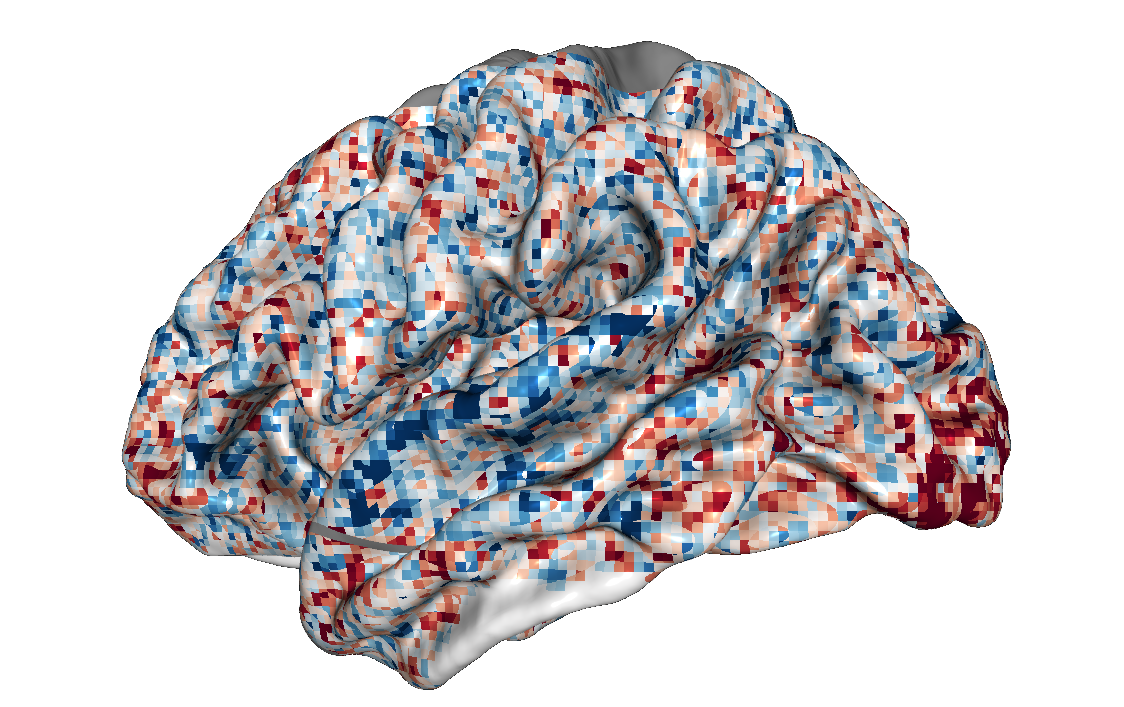
\includegraphics[scale=0.3]{figures/neuroscience/spatial_map.png}
  \caption{Contrast ``sentence listening versus sentence reading'' computed from the fMRI data of one
    subject in the IBC dataset~\cite{ibc, ibc2}. This contrast was downloaded
    from neurovault~\cite{gorgolewski2015neurovault} (collection 2138 subject 1 session 0) .}
  \label{fig:ibc_contrast}
\end{figure}


While in this thesis, we always work with unthresholded contrast maps like the one in Figure~\ref{fig:hcp_contrast}, contrast maps
are usually thresholded to keep only activity that is significantly
different from zero.
The GLM model is called univariate since interactions between voxels are not
modeled.
Univariate methods are often criticized for their inability to
capture well correlations and interactions between brain-wide measurements.
This makes it difficult to precisely locate brain functions from brain maps. An approach to overcome this issue is to train classifiers to \emph{decode} brain maps, i.e to discriminate between different stimulus of task
types~\cite{shirer_decoding_2012,varoquaux_how_2014,loula_decoding_2018}. When linear classifiers are used, the weights of this classifiers localize the brain functions.
This approach can be more powerful, as classifiers take correlations between
voxels into account. Decoding is also popular for individual imaging-based diagnosis.

\section{Magneto electro encephalography (MEG)}
Most material in this section is inspired from the book of Riitta Hari and Aina
Puce~\cite{hari2017meg}.

\subsection{Principle of MEG}
When a neuron fires, it emits a current that generates a magnetic field. By
recording the magnetic field close to the skull, we gain insight on neural
activity.

A limiting factor is that the magnetic fields induced by neuronal currents are
extremely weak (on the order of $10 fT$) which is much lower than the ambient magnetic noise ($10^8 fT$). Therefore recordings are performed in a shielded room and extremely sensitive magnetometers are used.
The best current tools can measure the magnetic filed generated by approximately 50~000 neurons oriented in the same direction.

MEG recording device also include gradiometers in addition to magnetometers.
These are sensitive to the local variations of the magnetic field. However in our experiments, we only use the magnetometers data.

MEG has a temporal resolution on the order of the ms which is essentially the same as electroencephalography (EEG). This is much better than fMRI. The spatial
resolution is similar to that of EEG and is on the order of the centimeter.
In general the brain sources are slightly better localized in MEG since the
magnetic field is not affected by changes in conductivity in the head.


\subsection{Solving the inverse problem}
In order to locate activation from the brain measurements, we need to solve an inverse problem: what kind of sources can generate the magnetic field we
observe ? This section gives an overview of the sLORETA
method~\cite{pascual2002standardized} and is strongly inspired from the tutorial
of the authors~\cite{pascual2007discrete}.

From a vector describing the 3D current density inside the brain $\jb \in \RR^{3 \times v}$
($v$ is the number of voxels) we
can predict the magnetic field recorded by the sensors $\bb \in \RR^p$ ($p$ is the number of sensors) provided
we know how the magnetic field propagates through the brain by using Maxwell's
equation. This is called the \emph{forward model}. Models describing the
geometry of the head (head models) are used to provide an approximate solution for the forward model.
We have therefore
\begin{align}
  \bb = K \jb
  \label{eq:maxwell}
\end{align}
where $K \in \RR^{p \times 3v}$ is given by the head model.
$K$ can be seen as $K  = [K_1 \dots K_{v}]$ where $K_i \in \RR^{p \times 3}$ describes how voxel $i$ contributes to the measured magnetic field $\bb$.

Note that if $\bb$ and $K$ are given there is an infinite number of possible
$\jb$ so the inverse problem must be regularized in order to select a solution among all possible ones.
A common parametrization is to assume that:
\begin{align}
\jb(K_i) = (K_i^{\top} C K_i) \bb
\end{align}
for a symmetric matrix $C \in \RR^{p \times p}$ and $\jb(K_i)$ describes the current at voxel $i$.
In sLORETA, we have $C = (K K^{\top} + \alpha I)^{\dagger}$ where $\dagger$
represents Moore's pseudo inverse, $I$ is the identity matrix and $\alpha$ is an hyperparameter. 

Taking a point wise source $\ab \in \RR^{3}$ at voxel $j$
equation~\eqref{eq:maxwell} yields $\bb = K_j \ab$.
Then, $\| \jb(K_i) \|^2$ is maximum at $K_i=K_j$ showing that the method can correctly recover point sources.

\subsection{Preprocessing steps}
This section is inspired from the preprocessing recommandations
in~\cite{jas2018reproducible} and the book of Riitta Hari and Aina
Puce~\cite{hari2017meg}. 

\subsubsection{Temporal filtering}
Temporal filtering is usually done by during analogous filtering using a wide range of
frequency (typically from $0.01 Hz$ to $200Hz$.
A digital filtering is usually applied afterwards. A low-pass filtering with
cut-off frequency at $40 Hz$ is valuable as it is below the line frequency.

\subsubsection{Independent component analysis}
Independent component analysis (ICA) can be used to isolate artifacts due to
heart beating or muscle contraction. As will be seen in section~\ref{sec:ica}.
ICA extracts independent components from the data. The data can be cleaned by
removing components corresponding to artifacts~\cite{jung1998extended}.

\subsubsection{Maxwell filtering}
Maxwell filtering also called signal space separation
(SSS)~\cite{taulu2006spatiotemporal} identifies the contributions of the
magnetic field from brain sources outside the brain and removes it.
This decreases the effect of outside noise and even allows to scan subjects with
implanted stimulators.


\subsection{Experimental designs}
Two kinds of responses are generally studied in MEG: \emph{evoked response} and
\emph{event related} response.
The evoked response is observed when the subject is exposed to a short stimuli.
We typically repeat the experiment multiple times and average the subject
response over trials.
Another technique is to average signal with respect to some event such as eye
movement or utterance of a word. The recovered signal is then called
event-related response.

\subsection{MEG datasets}
\label{sec:meg:datasets}
In this section, we give examples of MEG datasets. These examples are used in
the rest of the thesis to evaluate the methods developed.

The \emph{Sinusoidal Phantom MEG} dataset uses data collected with a realistic head phantom, which is a plastic device mimicking real electrical brain components.
% 
Eight current dipoles positioned at different locations can be switched on or off.
% 
We only consider the 102 magnetometers.
% 
An epoch corresponds to 3\,s of MEG signals where a dipole is switched on for 0.4\,s with an oscillation at 20\,Hz and a peak-to-peak amplitude of 200\,nAm.
% 
We have access to $100$ epochs per dipole.
%
Maxwell filtering was applied on the data and a low pass filter with cut-off
frequency at 40 Hz.

The \emph{Elekta Phantom MEG} dataset also uses data collected with a realistic
head phantom and is available as part of the Brainstorm
application~\cite{tadel2011brainstorm}.
This dataset involves 32 different dipole locations. Like in the
\emph{sinusoidal phantom} we only
consider the 102 magnetometers and apply Maxwell filtering and a low pass filter
with cut-off 40 Hz. The dipoles emit a signal at either a strong, medium or low
amplitude yielding 3 datasets.
We use the dataset where the emitted signal is very strong to recover the true signal
by performing a PCA with 1 component.
Then we work with the dataset where the emitted signal is the weakest.
Each epoch corresponds to 301 samples and 20 epochs are available in total.

The \emph{CamCAN} dataset~\cite{shafto2014cambridge}
contains the MEG data of 647 different
subjects exposed to an audio-visual stimuli. More precisely, subjects are presented simultaneously an
auditory stimuli lasting 300ms at frequency 300, 600 or 1200 Hz  and a
checkerboard pattern lasting 34ms. 120 trials are available.

